%----------------------------------------------------%
%              ANALISIS DE REQUISITOS                %
%----------------------------------------------------%

\chapter{Análisis de Requisitos}
\label{analisis-de-requisitos}

\section{Requisitos no-funcionales}
\label{analisis-de-requisitos:no-funcionales}

La aplicación ha sido desarrollada con dos requisitos básicos:

\begin{itemize}
\item Que tenga mucha funcionalidad con el mínimo posible de \textit{clicks}.
\item Que para el alumno no suponga una distracción.
\end{itemize}

Asi pues se ha creado un diseño agradable que pretende tener mucha funcionalidad, especialmente en la vista de profesor. En la vista del alumno se ha minimizado el diseño y los elementos para que no existan distracciones importantes en clase.\\

\subsection{Requisitos de la interfaz}
\label{analisis-de-requisitos:no-funcionales:interfaz}

Para hacer más intuitiva la aplicación se han concretado unos colores e iconos específicos para cada tipo de ejercicio, de modo que sea fácil asociar una acción o estado mediante un color o un icono.

\begin{itemize}
\item Ejercicios activos: color rojo, pretendiendo indicar actividad, y un icono de un avión de papel, simbolizando un ejercicio que ha sido lanzado.
\item Ejercicios finalizados: color azul, indicando calma (ya hemos terminado), y un icono de una bandera de meta, simbolizando el fin.
\item Ejercicios preparados: color amarillo y un icono de un reloj, indicando que esto no se ha lanzado aun (viendo las aplicaciones móvil más utilizadas resulta intuitivo el significado del reloj).
\end{itemize}

Para las estadísticas se ha dejado el color verde y un icono de un gráfico de barras. El color azul se emplea para otros botones, sin usar ningún icono.\\

\section{Requisitos funcionales}
\label{analisis-de-requisitos:funcionales}

En este apartado se presentan los requisitos funcionales recogidos en interfaces de papel

Siguiendo las pautas fijadas por los requisitos no-funcionales se han realizado interfaces sencillas e intuitivas. Se le ha dado mucha importancia a la filosofia de "en pocos \textit{clicks}" que sigue la aplicación. Por tanto, ante todo, se han minimizado la cantidad de transiciones entre pantallas y el uso de excesivos botones para buscar mucha funcionalidad en pocos \textit{clicks}.\\

El resultado queda plasmado en estos modelos de requisitos (M-1) de cada objetivo de usuario (User Objective).\\

\subsection{Requisito común: Autenticación}
\label{analisis-de-requisitos:funcionales:p1}

\begin{figure}[H]
\begin{subfigure}[b]{0.5\textwidth}
	\centering
	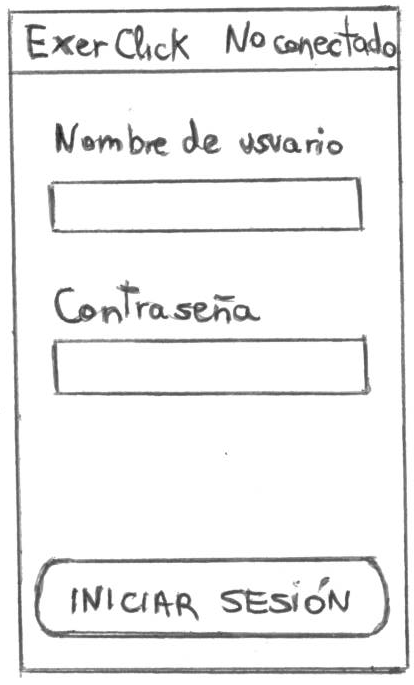
\includegraphics[height=7cm]{sheetprotos/p0}
	\caption{P0: Autenticación de usuario}
	\label{fig:req-autenticacion:p0}
\end{subfigure}
%
\begin{subfigure}[b]{0.5\textwidth}
	\centering
	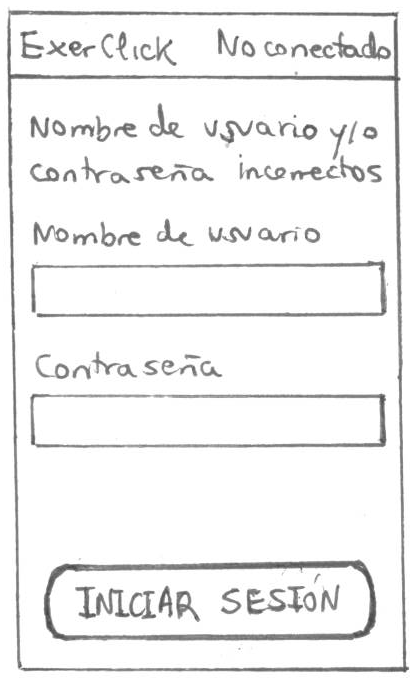
\includegraphics[height=7cm]{sheetprotos/p0'}
	\caption{P0': Error al introducir usuario o contraseña}
	\label{fig:req-autenticacion:p0'}
\end{subfigure}
%
\begin{subfigure}[b]{0.9\textwidth}
	\centering
	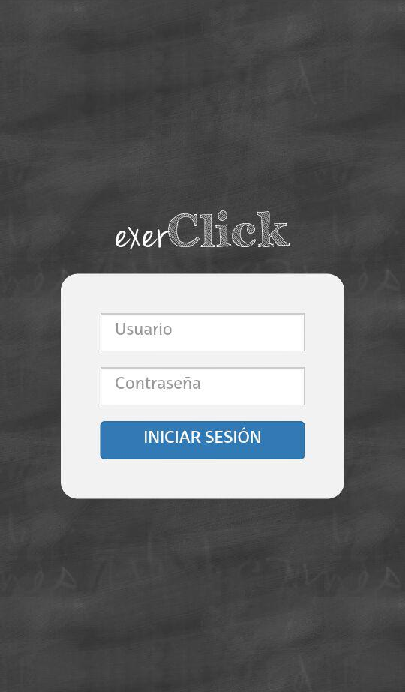
\includegraphics[width=0.5\textwidth]{fsm/autenticacion}
	\caption{Autómata de estados correspondiente a la Autenticación}
	\label{fig:fsm-autenticacion}
\end{subfigure}

\label{fig:autenticacion}
\end{figure}

La autenticación es un requisito común para todos los UOs. En su interfaz (P0) podemos ver dos campos para introducir nuestro nombre de usuario y contraseña y un botón para acceder. Si los datos son correctos veremos la interfaz P1 del profesor o del estudiante (dependiendo del tipo de usuario con el que no hayamos autenticado). De otro modo veremos la pantalla de error (P0').\\

En el autómata se muestra un bucle en el estado P0: cada vez que introducimos datos incorrectos nos muestra la pantalla de error (P0') y, en el caso del alumno, si no tuviera clase se nos muestra P0''. Tanto P0' como P0'' están derivadas de la interfaz P0 pero añadiendo un aviso de error.\\

\subsection{UO1-S: Responder a un ejercicio}
\label{analisis-de-requisitos:funcionales:uo1s}

\begin{figure}[H]
\begin{subfigure}[b]{0.5\textwidth}
	\centering
	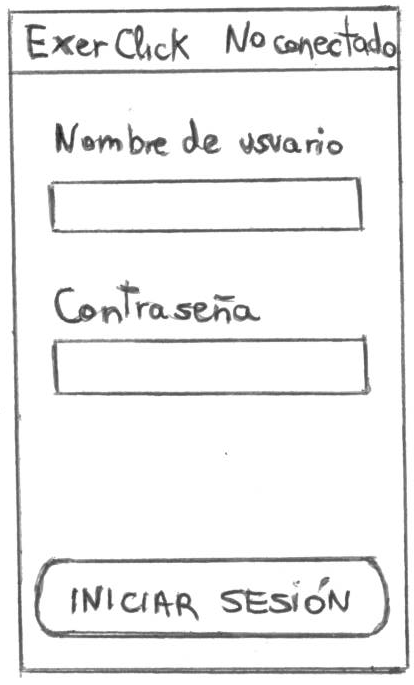
\includegraphics[height=7cm]{sheetprotos/p0}
	\caption{P6T: Sin filtro, se muestran todos los alumnos involucrados}
	\label{fig:files-css}
\end{subfigure}
%
\begin{subfigure}[b]{0.5\textwidth}
	\centering
	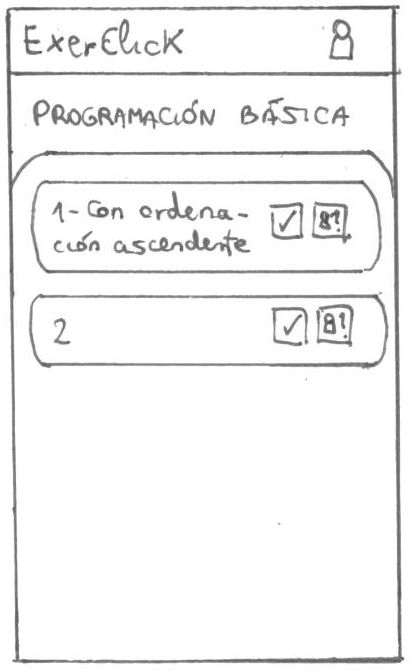
\includegraphics[height=7cm]{sheetprotos/student/p1}
	\caption{P6A: Sólo alumnos que hayan marcado el ejercicio como acabado}
	\label{fig:files-js}
\end{subfigure}

\begin{subfigure}[b]{\textwidth}
	\centering
	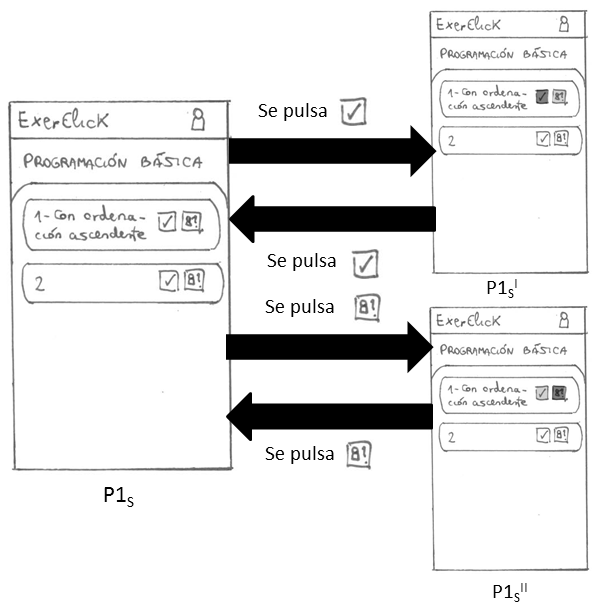
\includegraphics[width=0.5\textwidth]{fsm/uo1s}
	\caption{Autómata de estados correspondiente al UO1-S}
	\label{fig:fsm-uo1s}
\end{subfigure}

\label{fig:uo1s}
\end{figure}

El modelo M-1(1-S) cuenta con 2 pantallas. La primera (P0) sirve para autenticar al alumno en la aplicación (es una pantalla común a todos los UOs). Una vez se ha accedido a la pantalla principal del alumno (P1) podemos responder a los ejercicios indefinidamente sin cambiar de pantalla (tal y como demuestra el bucle en el autómata).\\

En el estado P1 nuestras opciones para responder a un ejercicio son marcar el ejercicio como finalizado (boton azul) o marcar una duda en el ejercicio (botón rojo).\\

\subsection{UO2-S: Ver la descripción completa de un ejercicio}
\label{analisis-de-requisitos:funcionales:uo2s}

\begin{figure}[H]
\begin{subfigure}[b]{0.5\textwidth}
	\centering
	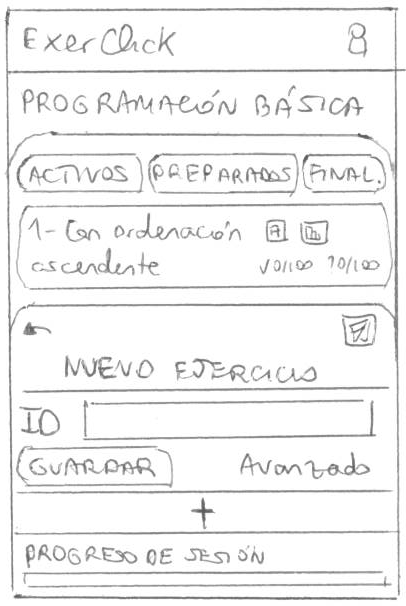
\includegraphics[height=7cm]{sheetprotos/student/p2}
	\caption{P2: }
	\label{fig:files-css}
\end{subfigure}


\label{fig:uo2s}
\end{figure}

Para acceder al M-1(2-S) es necesario pasar por P0 y P1. Haciendo \textit{click} sobre cualquier ejercicio (sobre la "caja") podremos acceder a P2. La interfaz se carga con datos sobre el ejercicio sobre el que hemos pinchado (identificador siempre y opcionalmente cualquier otro dato que el profesor haya incluido). Si no hubiera más detalles añadidos aparecerá un mensaje avisando de ello. El enlace "+Más" estaba pensado para mostrar más detalles sobre el ejercicio, aunque finalmente ha sido eliminado.\\

\subsection{UO1-T: Crear-Lanzar un ejercicio simple}
\label{analisis-de-requisitos:funcionales:uo1t}

\begin{figure}[H]
	\centering
	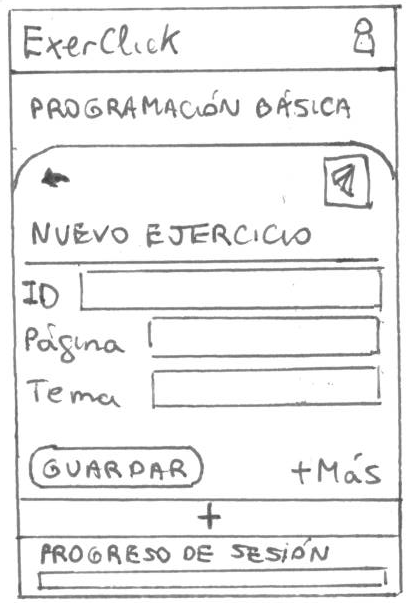
\includegraphics{sheetprotos/teacher/p2'}
	\caption{P2: Crear-Lanzar un ejercicio simple}
	\label{fig:p2-viejo}
\end{figure}

El M-1(1-T) cuenta con 3 pantallas: la de autenticación (P0), la principal del profesor (P1) y la pantalla para crear ejercicios nuevos (P2). P2 en un principio disponía  de 4 campos básicos para crear un ejercicio: un identificador, la página, el tema y una imagen. Todos los campos menos el identificador eran opcionales. Sin embargo, más tarde se pensó en reducir esto para que se viera más simple.\\

Tenemos 2 botones disponibles al igual que en la versión anterior: el de la parte superior (con un avión de papel) lanzará directamente el ejercicio como un ejercicio activo y el de la parte inferior guardará el ejercicio como ejercicio preparado para que podamos seguir editándolo antes de lanzarlo. Para guardar o lanzar un ejercicio es necesario que el campo del identificador no este vacío. Finalmente, disponemos de un enlace "Más" que nos llevará a la interfaz P2'.\\

\begin{figure}[H]
	\centering
	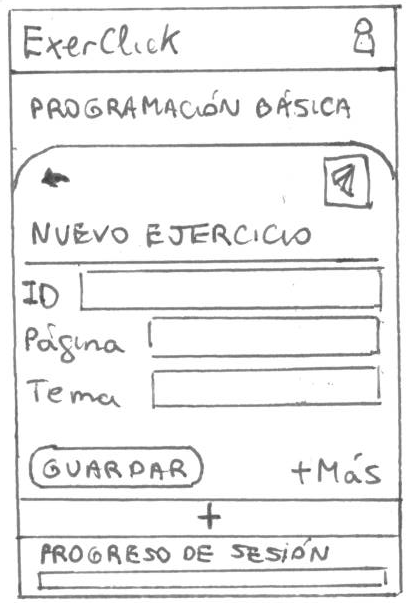
\includegraphics{sheetprotos/teacher/p2'}
	\caption{P2: Crear-Lanzar un ejercicio simple}
	\label{fig:p2}
\end{figure}

Esta nueva versión de la interfaz P2 utiliza la interfaz de P1 añadiendo una pestaña nueva en la que podremos crear un ejercicio simple. Estos ejercicios sólo necesitan de un identificador, por tanto, en esta pequeña pestaña sólo hay un campo para añadir ese identificador. Los campos omitidos pueden ser añadidos mediante el UO2-T. El enlace cambia de "Más" a "Avanzado" pero en cuanto a funcionalidad sigue siendo lo mismo.\\

\subsection{UO2-T: Crear-Lanzar un ejercicio detallado}
\label{analisis-de-requisitos:funcionales:uo2t}

\begin{figure}[H]
	\centering
	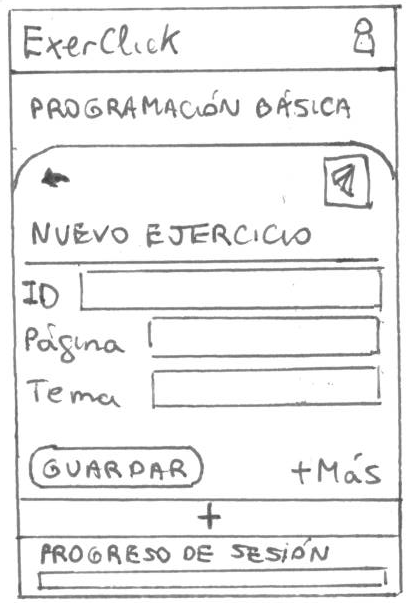
\includegraphics{sheetprotos/teacher/p2'}
	\caption{P2': Crear-Lanzar un ejercicio detallado}
	\label{fig:p2'}
\end{figure}

Este modelo M-1(2-T) es un modelo agregado de forma incremental al M-1(1-T). Es decir, tenemos que pasar por todo el modelo M-1(1-T), y finalmente podremos acceder a la interfaz P2' pulsando el enlace "Avanzado" en la interfaz P2. Los botones que aparecen siguen siendo los mismos que en P2. El enlace "Avanzado" cambia a "Menos", al pulsar en él volveremos a la interfaz P2. Todos los campos a excepción del identificador son opcionales.\\

\subsection{UO3-T: Cambiar el tipo de ejercicio}
\label{analisis-de-requisitos:funcionales:uo3t}

Este UO al principio tenía como finalidad cambiar un ejercicio de activo a finalizado (es decir, dar por finalizado un ejercicio propuesto en clase). Se cambió a cambiar el tipo de un ejercicio para volverlo más genérico (ya que se daba la posibilidad de cambiar de cualquier tipo a otro).\\

Este UO requiere de las pantallas P1A (ejercicios activos), P1F (ejercicios finalizados) y P1P (ejercicios propuestos). En un principio sólo existía un botón en los ejercicios activos para cambiar el ejercicios a finalizado. Luego se añadieron botones para poder realizar todas las combinaciones de cambios posibles.\\

\subsection{UO4-T: Ver estadísticas de un ejercicio}
\label{analisis-de-requisitos:funcionales:uo4t}

\begin{figure}[H]
\begin{subfigure}[b]{0.5\textwidth}
	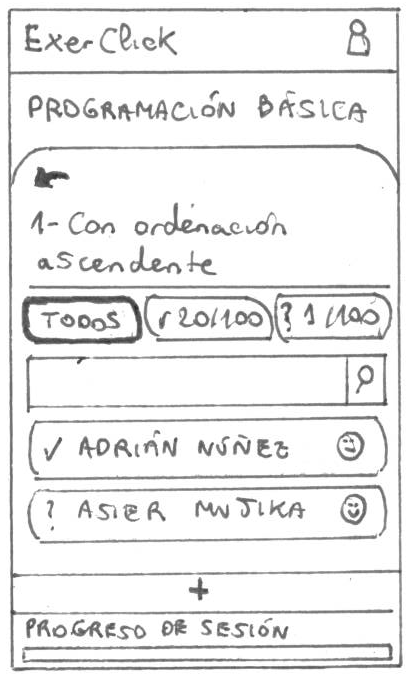
\includegraphics{sheetprotos/teacher/p5t}
	\caption{P5T: Sin filtro, se muestran todos los alumnos involucrados}
	\label{fig:p5t}
\end{subfigure}
%
\begin{subfigure}[b]{0.5\textwidth}
	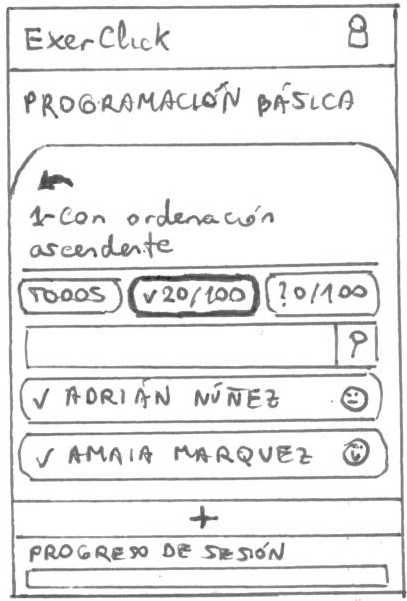
\includegraphics{sheetprotos/teacher/p5a}
	\caption{P5A: Sólo alumnos que hayan marcado el ejercicio como acabado}
	\label{fig:p5a}
\end{subfigure}

\label{fig:p5}
\end{figure}

El modelo M-1(4-T) está formado por 3 pantallas: P5T, P5A y P5D. Son necesarias 2 pantallas para acceder hasta estas: P0 y P1A o P1F (desde P1P es imposible).\\

\begin{itemize}
\item \textbf{P5T:} nos muestra a todos los alumnos involucrados en el ejercicios (que estén en la asignatura). Muestra también el estado de realización del ejercicio: acabado, con alguna duda o sin marcar nada.
\item \textbf{P5A:} nos filtra sólo los alumnos que han marcado el ejercicio como acabado.
\item \textbf{P5D:} igual que P5A pero marcando como duda el ejercicio.
\end{itemize}

Desde P1A o P1F siempre accederemos directamente a P5T y desde ésta podemos acceder a P5A y P5D mediante la pulsación de los botones de la parte superior (finalizados y en duda aparecen marcados con un icono representativo y el porcentaje de acabados/dudas respecto al número de alumnos).\\

\subsection{UO5-T: Ver la descripción completa de un ejercicio}
\label{analisis-de-requisitos:funcionales:uo5t}

\begin{figure}[H]
	\centering
	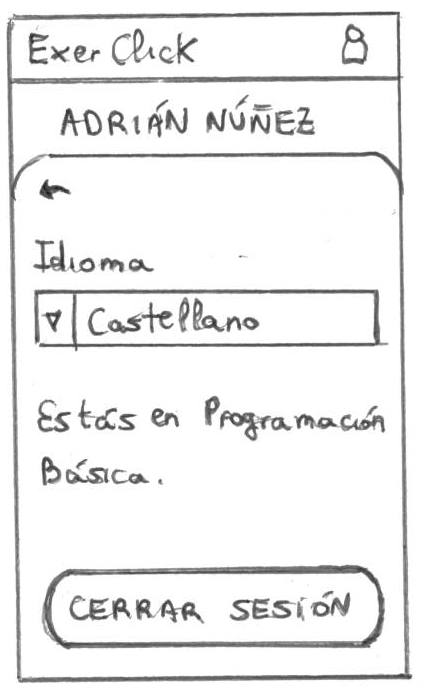
\includegraphics{sheetprotos/teacher/p3}
	\caption{P3: Se muestran los detalles de un ejercicio}
	\label{fig:p3}
\end{figure}

Para acceder al M-1(5-T) es necesario pasar por P0 y P1, y desde cualquier variante de P1 (P1A, P1F o P1P), haciendo \textit{click} sobre cualquier ejercicio (sobre la "caja") podremos acceder a P3. La interfaz se carga con datos sobre el ejercicio sobre el que hemos pinchado (identificador siempre y opcionalmente cualquier otro dato que hayamos introducido como profesor). Si no hubiera más detalles añadidos aparecerá un mensaje avisando de ello.\\

A diferencia del UO2-S (donde se mostraban también los detalles de un ejercicio) en P3 tenemos un botón con un engranaje en la parte superior, al pulsarlo nos llevará a P4 (editar el ejercicio). El enlace "+Más" sigue igual.\\

\subsection{UO6-T: Editar un ejercicio}
\label{analisis-de-requisitos:funcionales:uo6t}

El modelo M-1(6-T) es un modelo incremental del M-1(5-T), accederemos a el utilizando el botón con un engranaje que aparece en P3. Este modelo añade una nueva pantalla P4 desde la que podremos editar un ejercicio.\\

En la parte superior nos aparecerá el identificador del ejercicio (al principio como se ve aparecía más abajo, más tarde se hizo editable directamente en el título) y una flecha para ir hacia atrás. Esta flecha es más tarde eliminada, en su lugar aparece el botón de engranaje de nuevo como en P3. Este botón tendrá el mismo "efecto atrás" que la flecha.\\

En el centro tendremos campos para introducir nuevos valores para cada posible detalle de un ejercicio (sólo el identificador es obligatorio). Cuando queramos guardar los cambios habrá que pulsar el botón "Guardar". El enlace "Más" muestra más detalles que editar (aunque fue eliminado más adelante).\\

\subsection{UO7-T: Cerrar sesión}
\label{analisis-de-requisitos:funcionales:uo7t}

La última interfaz de la aplicación es P6. Esta interfaz es el perfil del profesor, donde se pueden realizar algunas opciones. Una de estas opciones es la de cerrar sesión. El modelo M-1(7-T) por tanto requiere de esta nueva interfaz P6, además de P0 y P1 (cualquier variante). Para acceder al perfil hay que hacer \textit{click} sobre el nombre de usuario de la parte superior de la aplicación. En P6, para cerrar sesión, tenemos que pulsar el botón "Cerrar sesión" de la parte inferior.\\

\subsection{UO8-T: Cambiar el idioma de la aplicación}
\label{analisis-de-requisitos:funcionales:uo8t}

Necesitamos nuevamente la interfaz P6 de la que depende el modelo M-1(8-T). En el perfil del profesor aparecerá una opción "Idioma" con un desplegable. Podemos escoger entre 4 idiomas: Castellano, Euskera, Inglés y Francés. Al escoger cualquiera la aplicación cambiará automáticamente de idioma.\\

\subsection{UO9-T: Cambiar de asignatura}
\label{analisis-de-requisitos:funcionales:uo9t}

El último UO depende de nuevo de la interfaz P6 para su modelo M-1(9-T). Existe otra opción con desplegable llamada "Asignatura", donde podremos escoger entre cualquier asignatura del profesor. Al escoger una nueva asignatura no se apreciarán más cambios que el texto que aparece sobre el botón de cerrar sesión (donde aparece la asignatura que está seleccionada), sin embargo la "asignatura activa" ha cambiado. Es decir, si volvemos de nuevo a los ejercicios (P1) veremos que estamos en la nueva asignatura seleccionada, y, por tanto, aparecerán los ejercicios de esa asignatura.\\

Para volver a P1 hay que pulsar la flecha "atrás". Más tarde se elimina y se sustituye por un botón "Ir a clase" en la parte superior.\\

\subsection{UO1: Lanzar ejercicios}
\label{analisis-de-requisitos:funcionales:uo1}

\subsection{UO2: Lanzar ejercicios y visualizar resultados}
\label{analisis-de-requisitos:funcionales:uo2}

\section{Requisitos de dispositivos para su ejecución}
\label{analisis-de-requisitos:dispositivos}

La aplicación está pensada para el uso en cualquier dispositivo móvil con los sistemas operativos Android e iOS. No está pensada para tamaños de pantalla excesivamente pequeños, donde probablemente la aplicación se vería incorrectamente.\\

En Android la versión mínima requerida es la 4.0 (API 15). En versiones 5.0 o superior no se garantiza que funcione correctamente.\\